\section{System}
The system uses two arrays, each with three microphones. Three microphones along with a micro-controller are mounted at three vertices of an equilateral triangle. Fig~\ref{fig:setup_array} shows a picture of the array. Micro-controller used in this project is \emph{teensy 3.1}. The micro-controller collects microphone data on all three channels for $12$ millisecond and then send the recorded data to a computer for localization. 

\begin{figure}[]
  \centering
  \begin{subfigure}[]{.2\textwidth}
    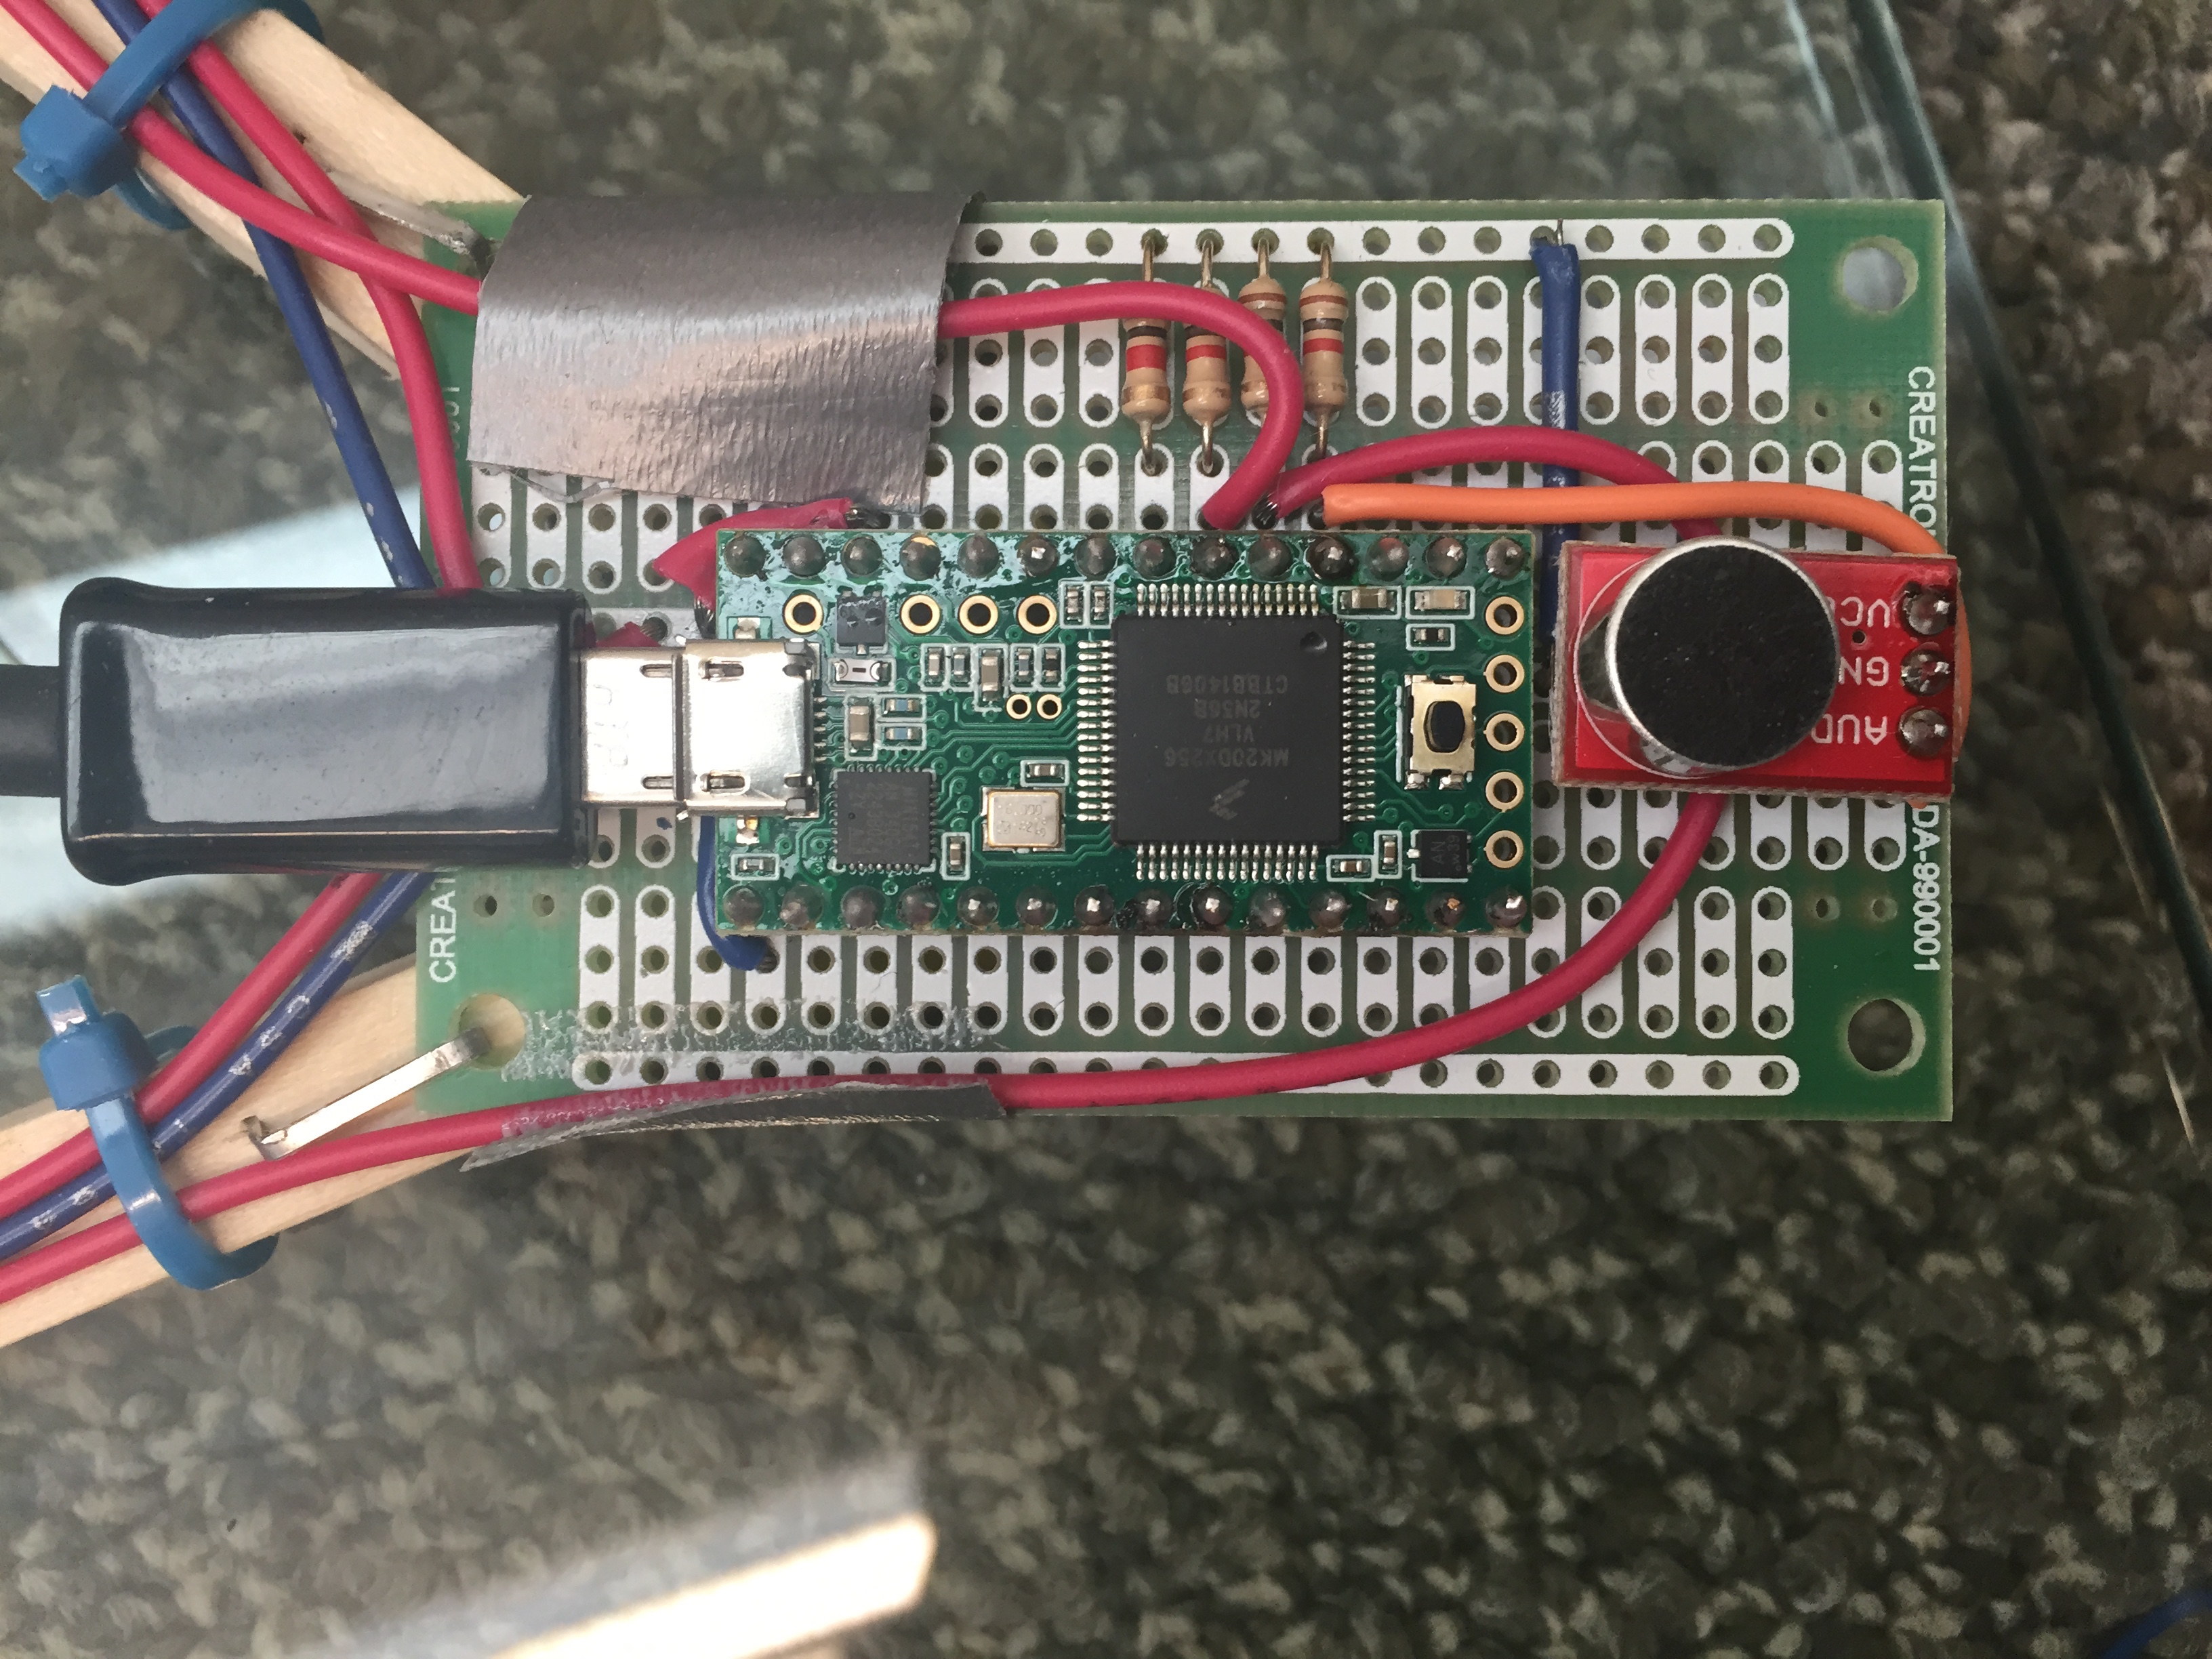
\includegraphics[width=\textwidth]{array_close.JPG}
  \end{subfigure}
  \begin{subfigure}[]{.2\textwidth}
    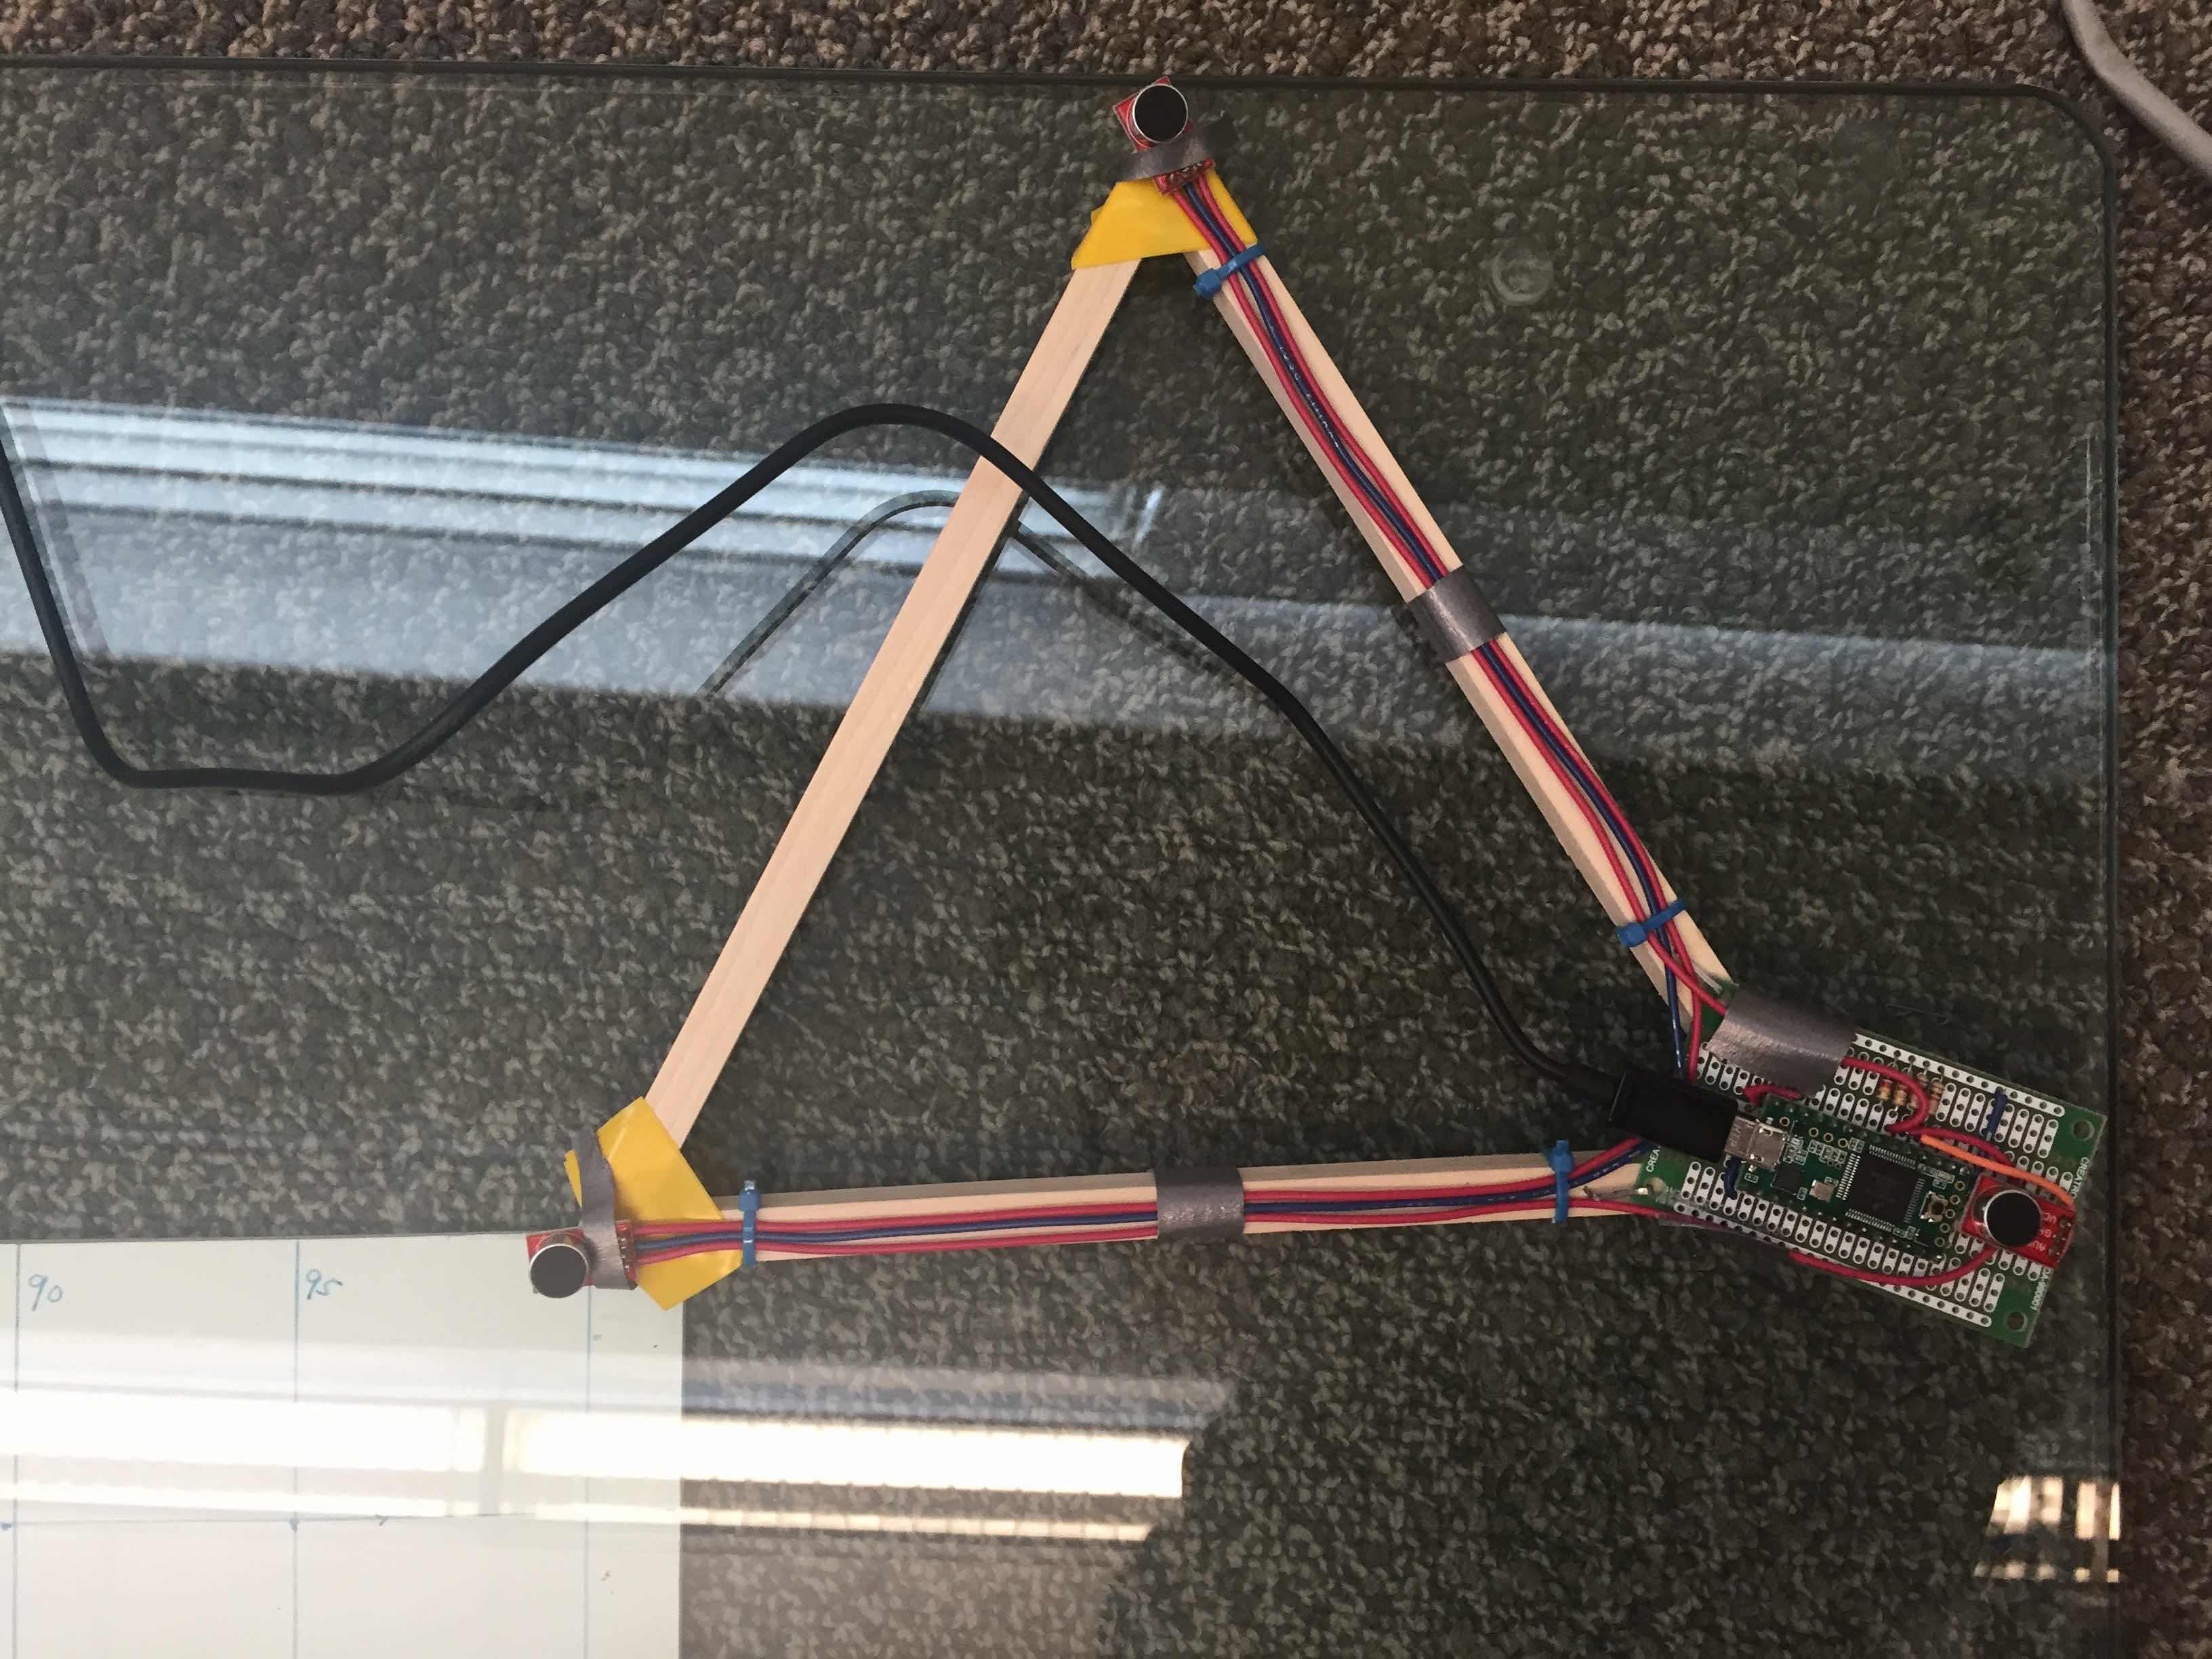
\includegraphics[width=\textwidth]{array.JPG}
  \end{subfigure}
  \caption{array}
  \label{fig:setup_array}
\end{figure}

From a timing point of view, the micro controller spends $12$ millisecond on sampling microphone data before sending the data to the computer for processing. Sending data through USB port takes another $18$ millisecond, and processing on computer takes around $50$ millisecond. Therefore, the totoal time lag between sound source and localization is around $80$ millisecond.
